\documentclass{article}
\usepackage[utf8]{inputenc}
\usepackage[T1]{fontenc}
\usepackage[french]{babel}
\usepackage{amsmath,amsfonts,amssymb,amsthm}
\usepackage[margin=2.5cm]{geometry}
\usepackage{graphicx}

\begin{document}

\paragraph{Introduction}
En ce qui concerne les diagrammes de séquence de l'extension de gestion de cartes. J'ai réaliser
ceux qui était les moins évident. Cependant ils suivent tous plus ou moins le même pattern.

\paragraph{Payer avec une carte}

Cette interaction comment par l'utilisateur qui entre les données nécessaires au paiement
dans la CardPayScene(1). La scène enclenche le payement à l'AbstractCard sélectionnée(2).
\newline
Ensuite:
\begin{itemize}
    \item Soit elle envoie sa demande de paiement(3). Le serveur répond qu'une erreur s'est produite.(4)
    La carte communique qu'une erreur s'est produite à la CardPayScene(5)
    \item Soit elle envoie sa demande de paiement(6). Le serveur répond que le transfer s'est correctement
        effectué. La carte communique que le paiement s'est effectué à la CardPayScene(5)
\end{itemize}
 


\begin{figure}[h!]
    \hbox{
        \centering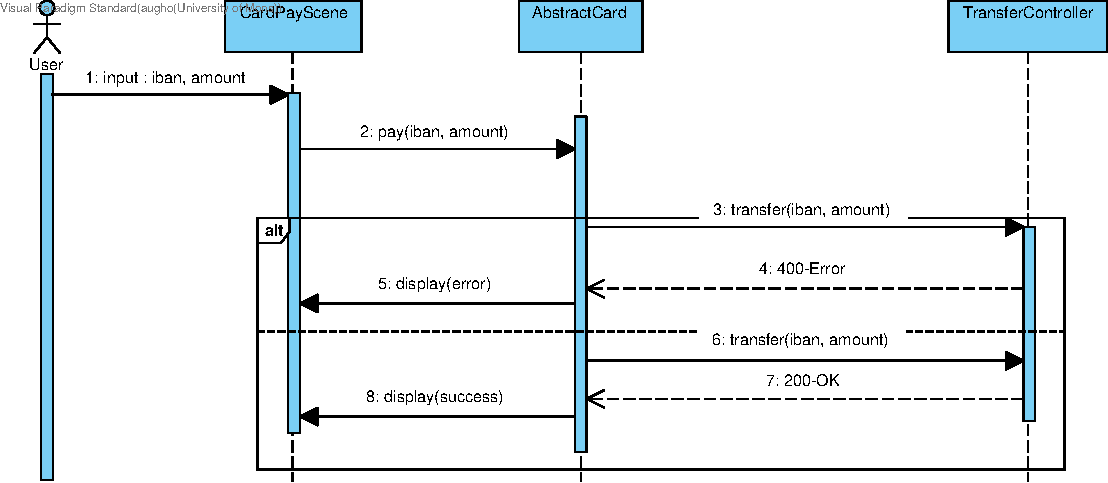
\includegraphics[width=\linewidth]{./img/sequence-client-Extension-1_pay.pdf}
    }
    \caption{Payer avec une carte}
\end{figure}

\newpage

\paragraph{Créer une carte}

Cette interaction comment par l'utilisateur qui entre les données nécessaires a la création
de la carte dans AddDebitCardScene(1). La scène crée la DebitCard basée sur ce que l'utilisateur
a entré(2).
\newline
Ensuite:
\begin{itemize}
    \item Soit elle envoie sa demande de création(3). Le serveur répond que la création s'est correctement
    effectuée(4). La carte communique que la création est validée à AddDebitCardScene(5)
    \item Soit elle envoie sa demande de création(6). Le serveur répond qu'une erreur s'est produite(7).
     La carte communique l'erreur à AddDebitCardScene(8)
\end{itemize}

\begin{figure}[h!]
    \hbox{
        \centering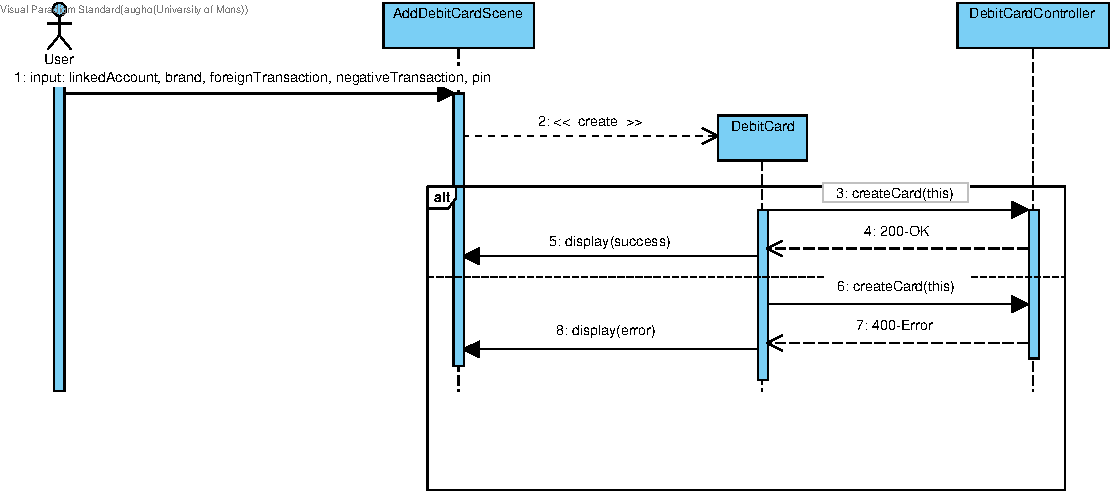
\includegraphics[width=\linewidth]{./img/sequence-client-Extension-1_create.pdf}
    }
    \caption{Créer une carte}
\end{figure}

\newpage

\paragraph{Modifier une carte}

Cette interaction comment par l'utilisateur qui entre les données nécessaires a la modification
de la carte dans DebitCardScene(1). La scène communique à DebitCard les données à modifier(2).
\newline
Ensuite:
\begin{itemize}
    \item Soit elle envoie sa demande de modification(3). Le serveur répond que la modification s'est correctement
    effectuée(4). La carte communique que la modification est validée à DebitCardScene(5)
    \item Soit elle envoie sa demande de modification(6). Le serveur répond qu'une erreur s'est produite(7).
     La carte communique l'erreur à DebitCardScene(8)
\end{itemize}

\begin{figure}[h!]
    \hbox{
        \centering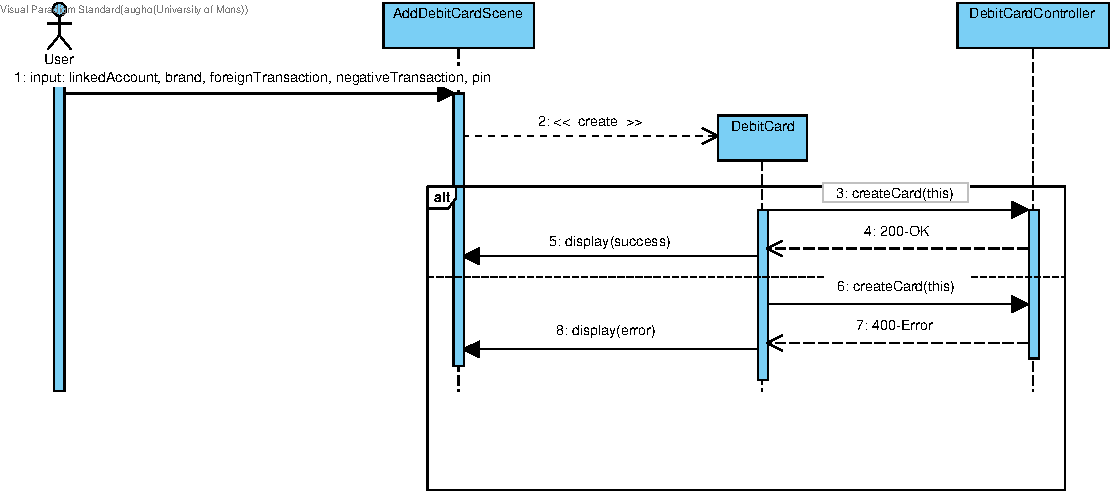
\includegraphics[width=\linewidth]{./img/sequence-client-Extension-1_create.pdf}
    }
    \caption{Modifier une carte}
\end{figure}

\end{document}